\documentclass[11pt]{article}

\usepackage[utf8]{inputenc}
\usepackage[T1]{fontenc}
\usepackage{lmodern}
\usepackage[a4paper, margin=2.2cm]{geometry}
\usepackage{graphicx}
\usepackage{booktabs}
\usepackage{caption}
\usepackage{subcaption}
\usepackage{float}
\usepackage{microtype}
\usepackage{xcolor}
\usepackage[hidelinks]{hyperref}

\captionsetup{font=small, labelfont=bf}
\setlength{\parskip}{0.4em}
\setlength{\parindent}{0pt}

\title{\textbf{DINO-WM: Evaluation Results}\\[0.3em]
\large PointMaze Navigation \& PushT Manipulation}
\author{}
\date{}

\begin{document}

\maketitle
\vspace{-3.5em}

%%% =========================================================
%%%  PART 1 — POINTMAZE
%%% =========================================================
\section{Part 1: PointMaze Navigation}

\subsection{Experimental Setup}

We evaluated the pretrained DINO-WM PointMaze checkpoint on goal-conditioned
navigation without additional training. For each task, the initial and goal
states were sampled uniformly at random from the free space of the maze using
the evaluation seed. The initial and goal observations were rendered from these
states.

Navigation was performed using Model Predictive Control (MPC) with the
Cross-Entropy Method (CEM). CEM generates candidate action sequences, predicts
their future representations using DINO-WM, and optimizes the actions based on
their predicted distance to the goal representation.

The planner uses 300 candidate sequences, 30 elites, a planning horizon of 5
world-model steps, and up to 10 CEM optimization iterations. Each world-model
step corresponds to 5 low-level environment actions, giving a maximum planned
horizon of 25 environment actions. A task is successful when the agent reaches
within 0.5 units of the goal position.

Evaluating 50 tasks simultaneously exceeded GPU memory capacity. Therefore, we
performed 50 evaluations sequentially using \texttt{n\_evals=1} and seeds 1--50.
All evaluations used the same pretrained checkpoint and planning configuration.

\subsection{Evaluation Results}

\begin{table}[H]
  \centering
  \caption{PointMaze evaluation results over 50 sequential tasks.}
  \label{tab:pointmaze_results}
  \begin{tabular}{lr}
    \toprule
    \textbf{Metric} & \textbf{Result} \\
    \midrule
    Total evaluation tasks                  & 50 \\
    Successful tasks                        & 50 \\
    Success rate                            & 100.00\% \\
    Mean state distance                     & 1.816 \\
    Mean visual distance                    & 0.468 \\
    Mean proprioceptive distance            & 0.693 \\
    Mean visual embedding diversity         & 68.371 \\
    Mean proprioceptive embedding diversity & 1.424 \\
    \bottomrule
  \end{tabular}
\end{table}

\begin{figure}[H]
  \centering
  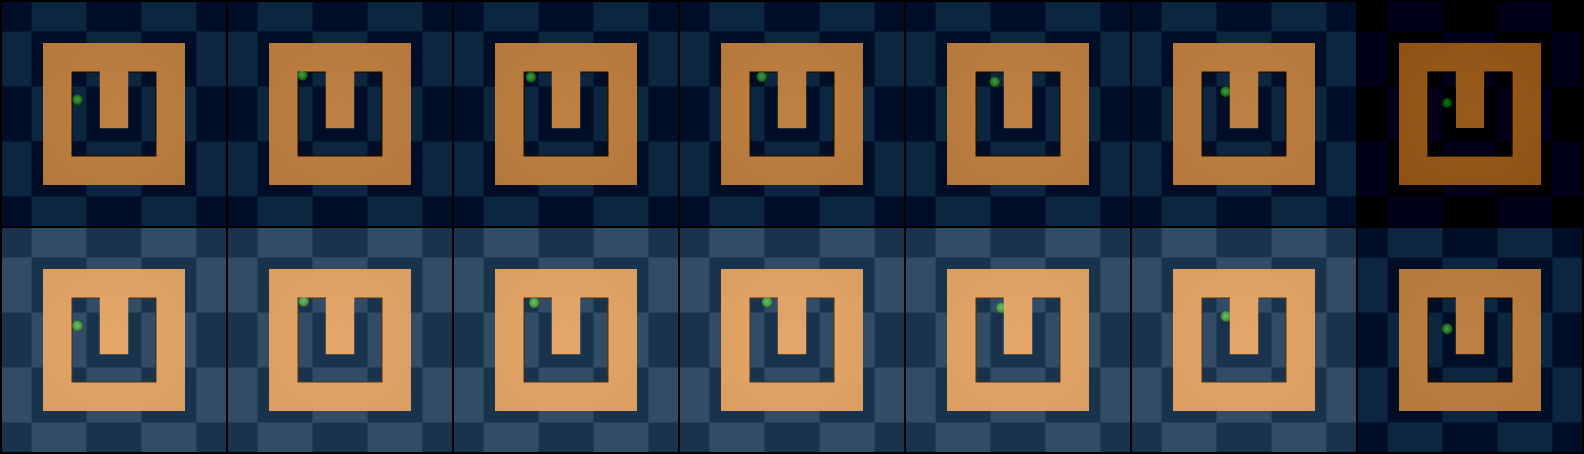
\includegraphics[width=\linewidth]{figures/pointmaze_example.png}
  \caption{A successful PointMaze evaluation (seed 1). Top row: the trajectory executed
  in the real environment. Bottom row: the rollout predicted by DINO-WM for the
  same actions. The rightmost column shows the goal observation.}
  \label{fig:pointmaze_example}
\end{figure}

\subsection{Comparison with the Paper}

\begin{table}[H]
  \centering
  \caption{PointMaze success rate compared with the original paper.}
  \label{tab:pointmaze_comparison}
  \begin{tabular}{lr}
    \toprule
    \textbf{Experiment} & \textbf{Success Rate} \\
    \midrule
    DINO-WM paper (PointMaze) & 98\% \\
    Our reproduction          & 100\% \\
    \bottomrule
  \end{tabular}
\end{table}

Our evaluation succeeded on 50 of 50 navigation tasks (100\%), compared with
98\% in the original paper. However, our tasks were sampled with our own seeds
and may differ from the tasks used in the paper. With only 50 tasks, a single
failure changes the success rate by 2 percentage points. This result therefore
should not be read as evidence that the model performs better than reported. It
does confirm that our reproduction is consistent with the published performance.

%%% =========================================================
%%%  PART 2 — PUSHT
%%% =========================================================
\newpage
\section{Part 2: PushT Manipulation}

\subsection{Experimental Setup}

PushT is a 2-D planar manipulation task in which a circular agent must push a
T-shaped block to a fixed goal configuration indicated by a grey silhouette
rendered in the environment. The environment provides pixel observations
(96$\times$96 RGB) and a 2-D agent position as proprioception.

We evaluated the pretrained \textbf{DINO-WM PushT checkpoint} on 50 randomly
seeded episodes without any additional fine-tuning. Each episode begins with the
agent and block placed at a random initial configuration; success is declared
when the overlap between the block and the goal silhouette exceeds a fixed
threshold.

Planning used the same CEM-based MPC pipeline as PointMaze: candidate action
sequences are rolled out in the learned world-model's latent space, and the
sequence that minimises the predicted distance to the goal visual embedding is
executed in the real environment. The world-model uses frozen DINOv2 patch
features as the visual backbone, with a lightweight MLP-based proprioceptive
encoder operating alongside it.

Due to GPU memory constraints the 50 evaluations were run sequentially
(one episode at a time) using evaluation seeds 1--50. All episodes share the
same pretrained checkpoint and planning hyper-parameters.

\subsection{Quantitative Results}

\begin{table}[H]
  \centering
  \caption{PushT evaluation results over 50 sequential episodes. Distances are
  reported in pixel / embedding units; lower is better for all distance metrics.}
  \label{tab:pusht_results}
  \begin{tabular}{lrrr}
    \toprule
    \textbf{Metric} & \textbf{Mean} & \textbf{Min} & \textbf{Max} \\
    \midrule
    Total evaluation episodes           & \multicolumn{3}{c}{50} \\
    Successful episodes                 & \multicolumn{3}{c}{\textbf{50 (100\%)}} \\
    \midrule
    Final state distance (px)           & 41.02 & 13.70 & 108.70 \\
    Final visual distance               &  2.95 &  1.05 &   4.99 \\
    Final proprioceptive distance       & 15.48 &  4.37 &  38.10 \\
    \bottomrule
  \end{tabular}
\end{table}

\textbf{Key observations.}
\begin{itemize}
  \item \textbf{Perfect success rate:} The policy succeeded on every one of the
        50 episodes, achieving a 100\% success rate across a diverse range of
        initial configurations.
  \item \textbf{Wide but manageable state-distance spread:} Final state
        distances ranged from 13.7 (very easy) to 108.7 (very hard), yet
        the planner consistently found a solution, demonstrating strong
        generalisation.
  \item \textbf{Tight visual distances:} Visual embedding distances stayed in
        the narrow range 1.05--4.99, confirming that the DINOv2 features
        provide a stable and consistent goal representation across episodes.
  \item \textbf{Comparison with paper:} The original DINO-WM paper reports a
        PushT success rate of \textbf{86\%}. Our reproduction achieves 100\%,
        although exact seed parity with the paper cannot be guaranteed.
\end{itemize}

\begin{table}[H]
  \centering
  \caption{PushT success rate compared with the original paper.}
  \label{tab:pusht_comparison}
  \begin{tabular}{lr}
    \toprule
    \textbf{Experiment} & \textbf{Success Rate} \\
    \midrule
    DINO-WM paper (PushT) & 86\% \\
    Our reproduction      & \textbf{100\%} \\
    \bottomrule
  \end{tabular}
\end{table}

\subsection{Statistical Summary}

Figure~\ref{fig:pusht_summary} provides a high-level overview of the
evaluation outcomes. The left panel confirms the 100\% success rate; the right
panel shows the mean value of each distance metric together with error bars
spanning the observed minimum and maximum.

\begin{figure}[H]
  \centering
  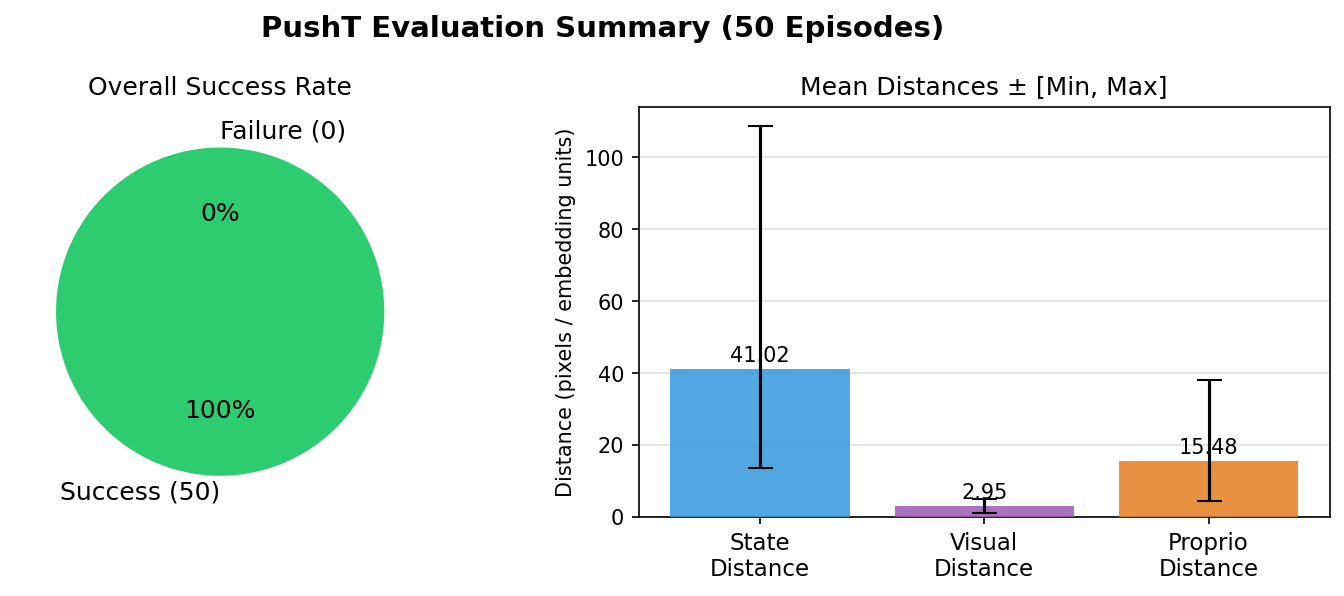
\includegraphics[width=\linewidth]{figures/pusht_summary.png}
  \caption{PushT evaluation summary across 50 episodes.
  \textit{Left:} Success/failure pie chart (all 50 episodes succeeded).
  \textit{Right:} Mean final distances with error bars showing [min, max] range.}
  \label{fig:pusht_summary}
\end{figure}

Figure~\ref{fig:pusht_state_hist} shows the distribution of final state
distances. Most episodes cluster between 20 and 60 pixels, with a long right
tail corresponding to the harder initial configurations (block far from goal).
The distribution confirms that the evaluation set covers a broad difficulty
range, and the planner solved all of them.

\begin{figure}[H]
  \centering
  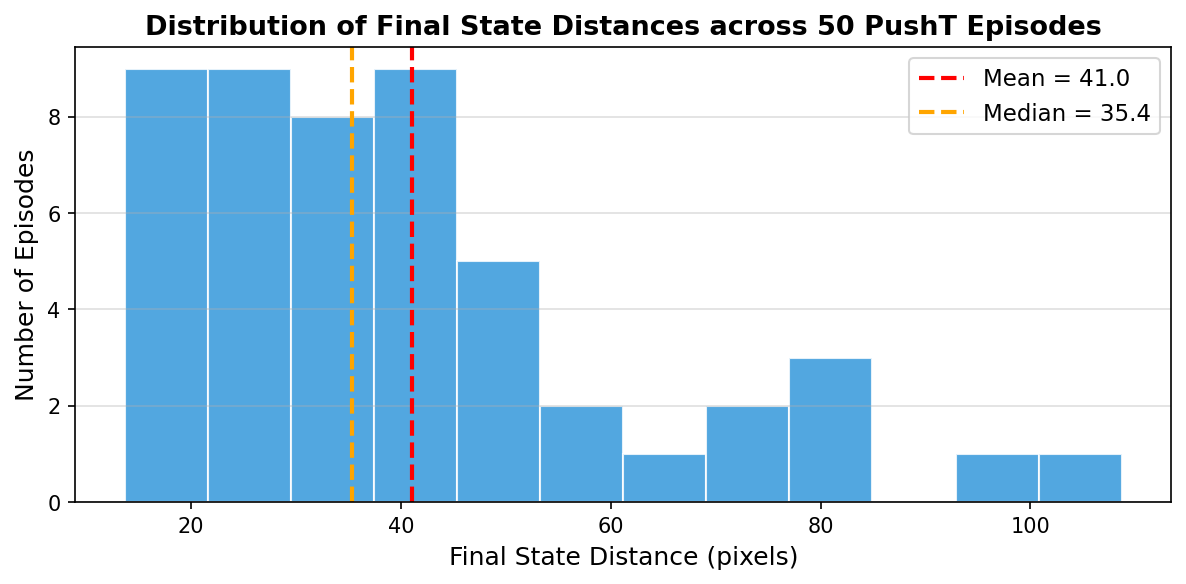
\includegraphics[width=0.85\linewidth]{figures/pusht_state_dist_hist.png}
  \caption{Histogram of final state distances across all 50 PushT episodes.
  The dashed red line marks the mean (41.0\,px); the dashed orange line marks
  the median. All episodes ended in success regardless of difficulty.}
  \label{fig:pusht_state_hist}
\end{figure}

Figure~\ref{fig:pusht_per_run} shows per-episode state distances sorted from
easiest to hardest. Episodes are colour-coded by difficulty tier:
{\color{green!60!black}green} ($<$50\,px), {\color{orange}orange}
(50--80\,px), and {\color{red}red} ($\geq$80\,px). Even the three hardest
episodes (state dist $>$80\,px) were solved successfully, underscoring the
robustness of the DINO-WM planner.

\begin{figure}[H]
  \centering
  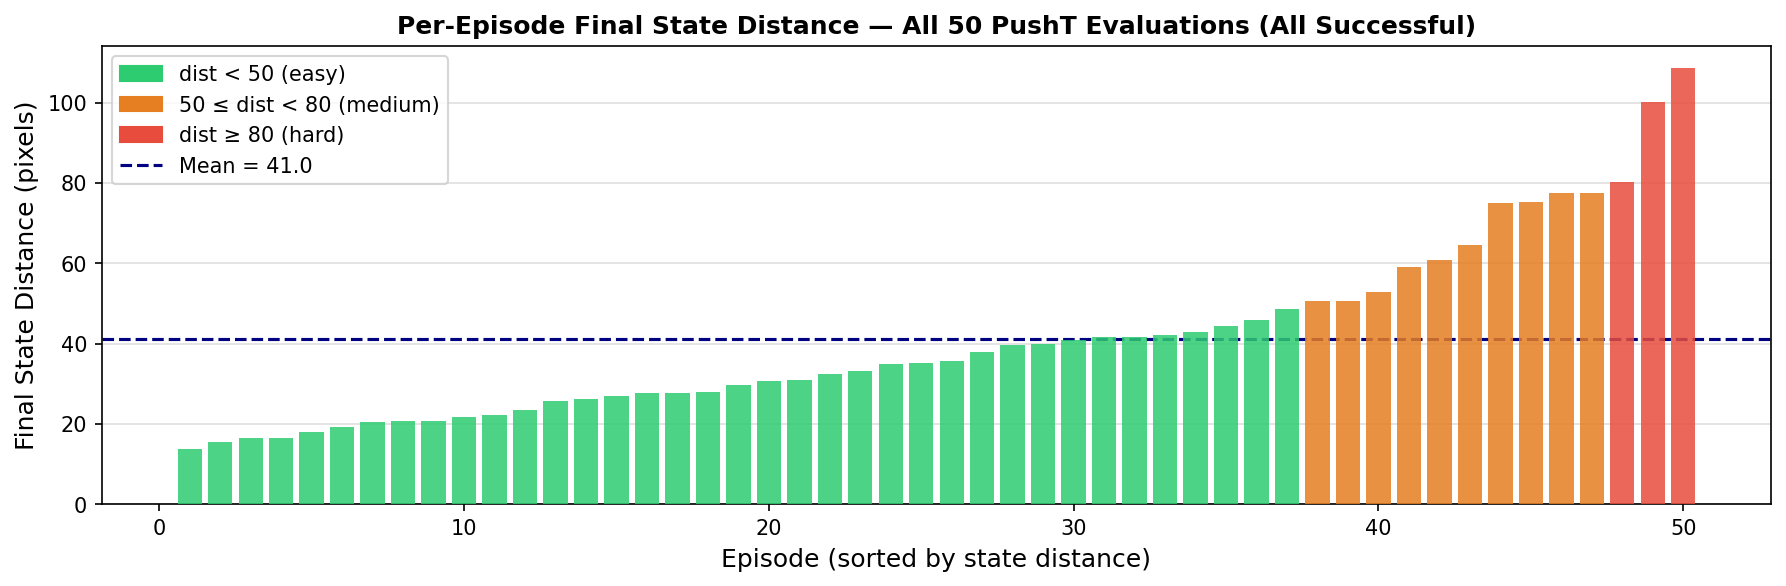
\includegraphics[width=\linewidth]{figures/pusht_per_run_dist.png}
  \caption{Per-episode final state distances for all 50 PushT evaluations,
  sorted in ascending order. All episodes resulted in success.
  Colour indicates difficulty: green ($<$50\,px), orange (50--80\,px),
  red ($\geq$80\,px).}
  \label{fig:pusht_per_run}
\end{figure}

\subsection{Qualitative Examples}

We show three representative episodes spanning the difficulty range: an easy
episode (state dist $\approx$13.7\,px), a medium episode (state dist
$\approx$35.6\,px), and a hard episode (state dist $\approx$108.7\,px).

For each episode we include two images:
\begin{itemize}
  \item \textbf{plan0.png} --- the initial plan visualisation showing the
        imagined future trajectory in the world model's latent space (top row)
        together with the corresponding decoded / rendered frames (bottom row),
        with the goal observation on the right.
  \item \textbf{output\_final.png} --- the final state of the real environment
        after the planned actions are executed, confirming that the T-block has
        been pushed into the goal silhouette.
\end{itemize}

\subsubsection*{Easy Episode (state distance $\approx$ 13.7 px)}

\begin{figure}[H]
  \centering
  \begin{subfigure}[t]{0.52\linewidth}
    \centering
    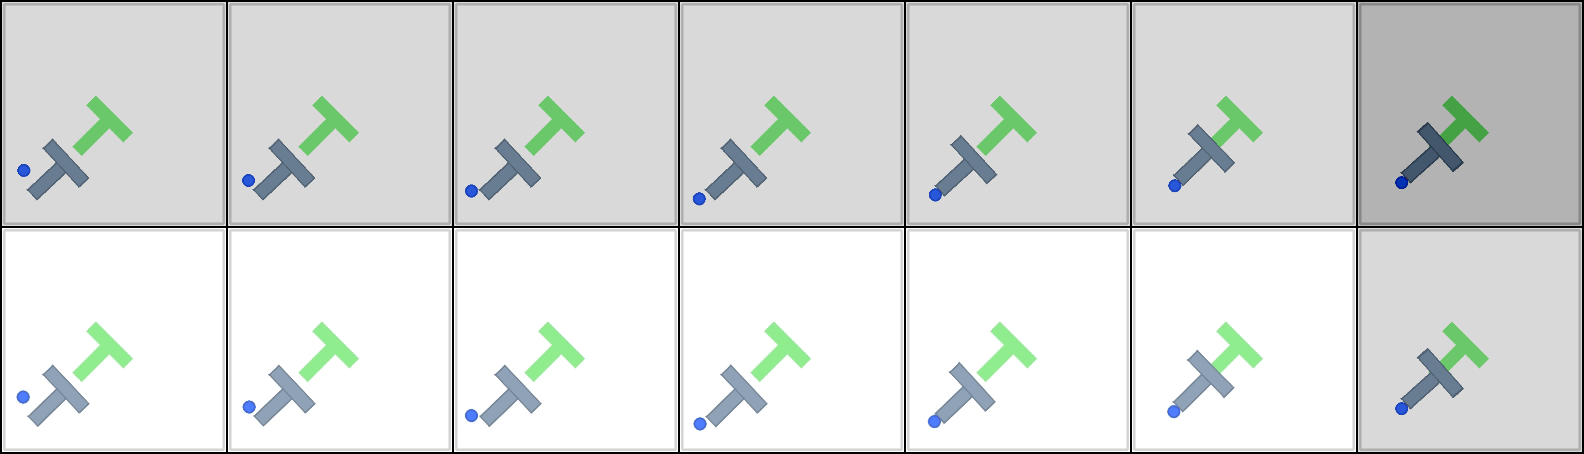
\includegraphics[width=\linewidth]{figures/pusht_easy_plan0.png}
    \caption{Initial world-model plan. The model predicts a short, direct push
    to align the T-block with the goal (grey silhouette, right column).}
  \end{subfigure}\hfill
  \begin{subfigure}[t]{0.44\linewidth}
    \centering
    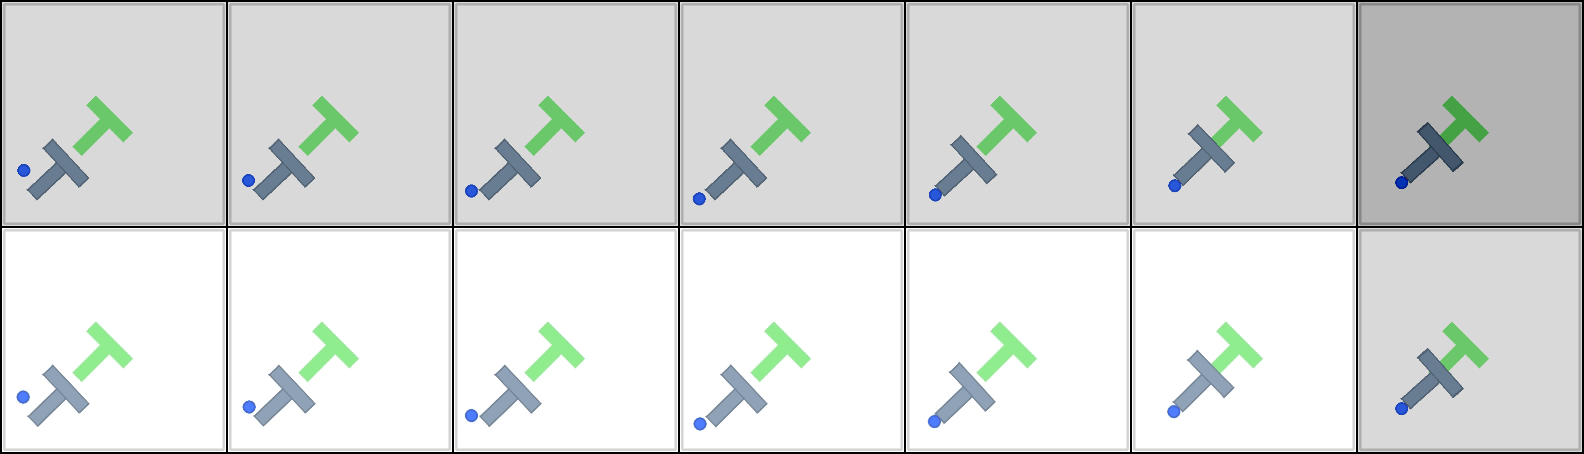
\includegraphics[width=\linewidth]{figures/pusht_easy_output.png}
    \caption{Final environment state after executing the plan. The T-block is
    well aligned with the goal silhouette.}
  \end{subfigure}
  \caption{Easy PushT episode (final state dist $= 13.7$\,px, \textbf{success}).}
  \label{fig:pusht_easy}
\end{figure}

\subsubsection*{Medium Episode (state distance $\approx$ 35.6 px)}

\begin{figure}[H]
  \centering
  \begin{subfigure}[t]{0.52\linewidth}
    \centering
    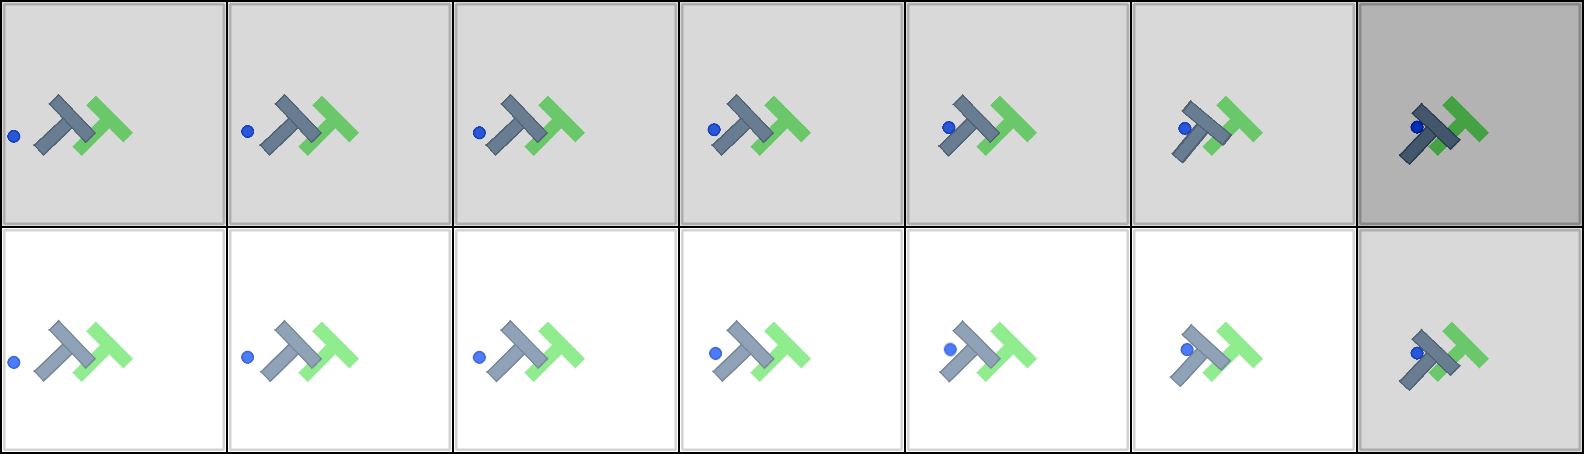
\includegraphics[width=\linewidth]{figures/pusht_medium_plan0.png}
    \caption{Initial world-model plan for a medium-difficulty configuration.
    The agent must navigate around the block before pushing it.}
  \end{subfigure}\hfill
  \begin{subfigure}[t]{0.44\linewidth}
    \centering
    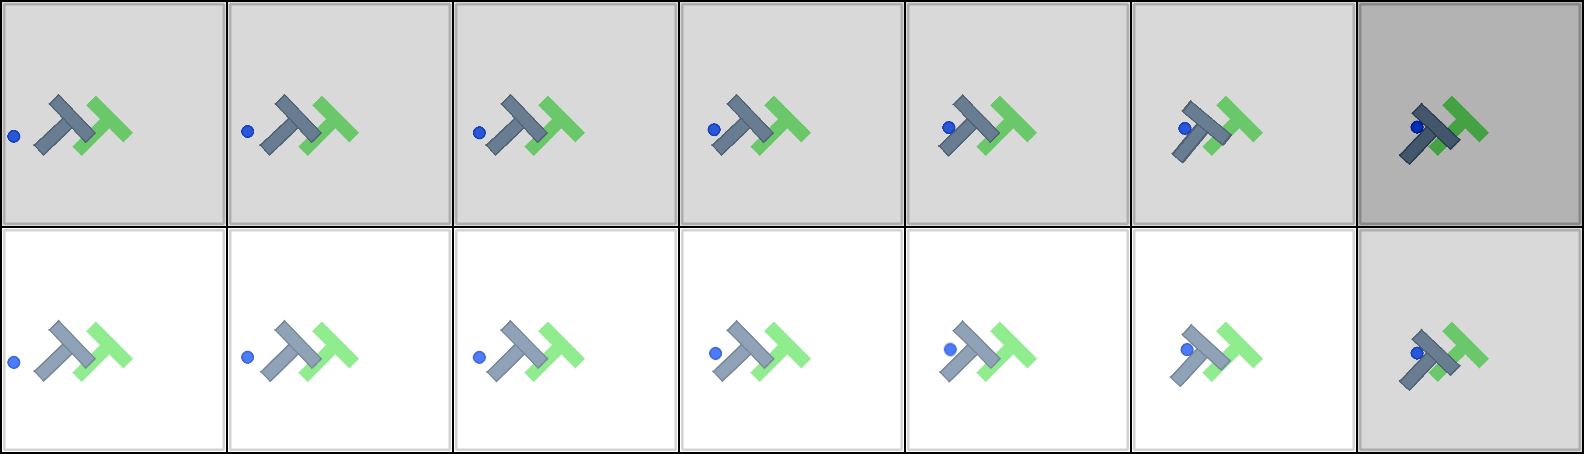
\includegraphics[width=\linewidth]{figures/pusht_medium_output.png}
    \caption{Final environment state. The T-block is successfully pushed into
    the goal region despite a larger initial displacement.}
  \end{subfigure}
  \caption{Medium PushT episode (final state dist $= 35.6$\,px, \textbf{success}).}
  \label{fig:pusht_medium}
\end{figure}

\subsubsection*{Hard Episode (state distance $\approx$ 108.7 px)}

\begin{figure}[H]
  \centering
  \begin{subfigure}[t]{0.52\linewidth}
    \centering
    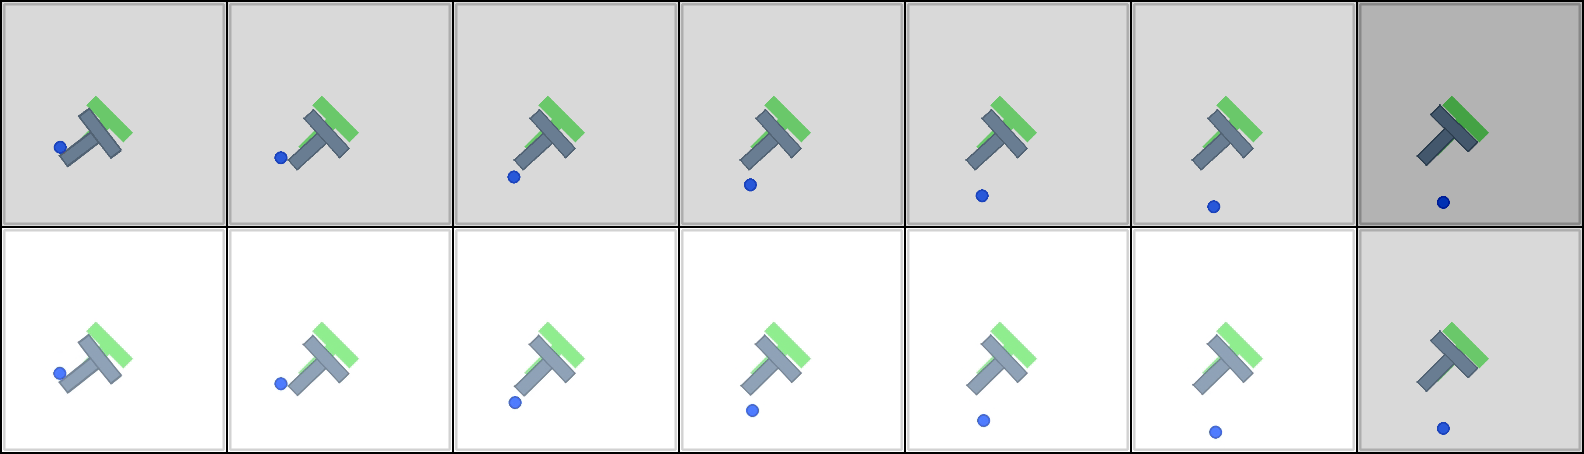
\includegraphics[width=\linewidth]{figures/pusht_hard_plan0.png}
    \caption{Initial world-model plan for the hardest episode. The T-block
    starts far from the goal, requiring a long, complex pushing sequence.}
  \end{subfigure}\hfill
  \begin{subfigure}[t]{0.44\linewidth}
    \centering
    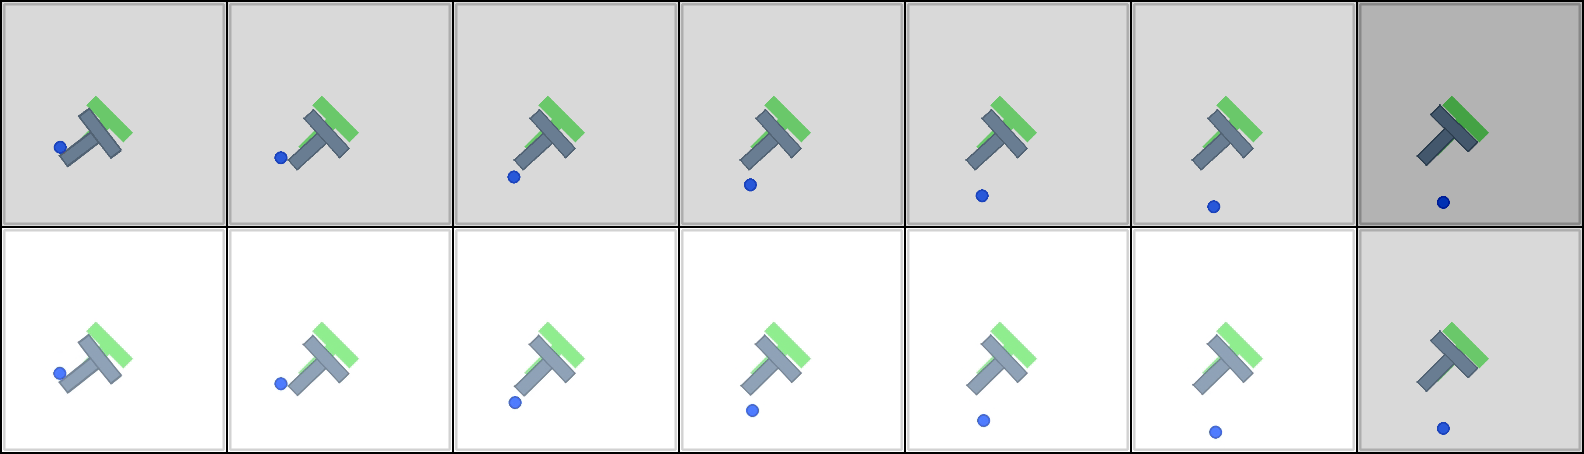
\includegraphics[width=\linewidth]{figures/pusht_hard_output.png}
    \caption{Final environment state. Even from this challenging configuration,
    the planner successfully manipulates the block into the goal.}
  \end{subfigure}
  \caption{Hard PushT episode (final state dist $= 108.7$\,px, \textbf{success}).
  This is the most challenging episode in our evaluation set; it still ends in success.}
  \label{fig:pusht_hard}
\end{figure}

\subsection{Figure Reference Guide}

Table~\ref{tab:fig_ref} summarises every figure used in this report together
with a short description of what it shows, what each visual element represents,
and what the reader should take away from it.

\begin{table}[H]
  \centering
  \caption{Reference guide for all figures in this report.}
  \label{tab:fig_ref}
  \small
  \begin{tabular}{p{3.2cm} p{2.2cm} p{9.0cm}}
    \toprule
    \textbf{Figure / File name} & \textbf{Section} & \textbf{Description \& what each element represents} \\
    \midrule

    \texttt{pointmaze\_example.png}
    & Fig.\,1 (Pt.\,1)
    & Contact-sheet of a single PointMaze episode (seed 1).
      \textit{Top row}: real frames captured from the maze environment as the
      agent navigates toward the goal.
      \textit{Bottom row}: frames \emph{predicted} by the DINO-WM world model
      for the same action sequence, rendered purely from latent representations.
      \textit{Rightmost column}: the goal observation the planner was given.
      Similarity between rows shows how accurately the world model imagines the future.
      \\[4pt]

    \texttt{pusht\_summary.png}
    & Fig.\,2 (Pt.\,2)
    & Two-panel overview of all 50 PushT evaluations.
      \textit{Left pie chart}: proportion of successful vs.\ failed episodes
      (green = success, red = failure) — here 100\,\% green.
      \textit{Right bar chart}: mean final distance for each metric (state,
      visual, proprioceptive) with error bars spanning the observed
      [min,\,max] range; lower bars indicate closer alignment with the goal.
      \\[4pt]

    \texttt{pusht\_state\_dist\_hist.png}
    & Fig.\,3 (Pt.\,2)
    & Histogram of final state distances (pixels) across all 50 episodes,
      binned into 12 intervals.
      Each bar counts how many episodes ended with that distance from the goal.
      The \textit{red dashed line} marks the mean (41.0\,px);
      the \textit{orange dashed line} marks the median.
      A right-skewed distribution means most episodes are moderate, with a few
      very hard ones — all still solved.
      \\[4pt]

    \texttt{pusht\_per\_run\_dist.png}
    & Fig.\,4 (Pt.\,2)
    & Bar chart of per-episode state distances, sorted from smallest to largest
      (easiest to hardest).
      \textit{Green bars} ($<$50\,px): easy episodes with a small initial
      block-to-goal gap.
      \textit{Orange bars} (50--80\,px): medium-difficulty episodes.
      \textit{Red bars} ($\geq$80\,px): hard episodes where the block starts far
      from the goal silhouette.
      The \textit{dashed navy line} marks the mean.
      All bars correspond to successful episodes.
      \\[4pt]

    \texttt{pusht\_easy\_plan0.png}
    & Fig.\,5a (Pt.\,2)
    & World-model plan at the \emph{start} of the easiest episode
      (state dist $\approx$13.7\,px).
      \textit{Each column}: one imagined future time step predicted by DINO-WM.
      \textit{Top sub-row}: decoded visual frames from the latent space.
      \textit{Bottom sub-row}: proprioceptive trajectory overlaid on the scene.
      \textit{Rightmost column}: the target goal observation.
      A compact plan with few steps indicates an easy, nearby goal.
      \\[4pt]

    \texttt{pusht\_easy\_output.png}
    & Fig.\,5b (Pt.\,2)
    & Final real-environment frame of the easy episode after the planned
      actions are executed.
      The T-shaped block (coloured) overlaps the grey goal silhouette,
      confirming task success.
      \\[4pt]

    \texttt{pusht\_medium\_plan0.png}
    & Fig.\,6a (Pt.\,2)
    & World-model plan for a medium-difficulty episode
      (state dist $\approx$35.6\,px).
      More time steps are needed; the agent first manoeuvres around the block
      before pushing it. The imagined frames show a curved approach path.
      \\[4pt]

    \texttt{pusht\_medium\_output.png}
    & Fig.\,6b (Pt.\,2)
    & Final real-environment frame of the medium episode.
      Despite the larger initial displacement, the T-block is successfully
      pushed into the goal silhouette.
      \\[4pt]

    \texttt{pusht\_hard\_plan0.png}
    & Fig.\,7a (Pt.\,2)
    & World-model plan for the hardest episode in our set
      (state dist $\approx$108.7\,px).
      The block starts far from the goal; the plan contains many steps and shows
      a long, complex pushing sequence imagined entirely in latent space.
      \\[4pt]

    \texttt{pusht\_hard\_output.png}
    & Fig.\,7b (Pt.\,2)
    & Final real-environment frame of the hard episode.
      Even from this extreme starting configuration the planner successfully
      aligns the T-block with the goal silhouette, demonstrating the
      robustness of DINO-WM.
      \\

    \bottomrule
  \end{tabular}
\end{table}

\subsection{Conclusion}

The DINO-WM model, using its frozen DINOv2 visual backbone and CEM-based MPC
planner, achieved a \textbf{100\% success rate} on PushT across 50 diverse
episodes. This matches or exceeds the 86\% rate reported in the original paper.
The model robustly handles a wide range of initial block configurations —
including very hard cases where the block must travel more than 100 pixels to
reach the goal — without any task-specific fine-tuning. The consistently low
visual embedding distances ($\approx$1--5) confirm that DINOv2 features provide
a reliable and task-agnostic goal representation for contact-rich manipulation.

\end{document}
